\section{Platinenaufbau}
Die Platine ist mit mehreren Bauteilen ausgestattet, die bis auf drei selbst zu dimensionierende Widerstände bereits vollständig bestückt ist.

Zur Erklärung von Abbildung 4.1 hier eine kurze Information zu den wichtigsten Abkürzungen:
\begin{itemize}
    \item R: Widerstand
    \item C: Kondensator
    \item J: Stecker/Relais
\end{itemize}

Die wichtigsten Bauteile sind:
\begin{itemize}
    \item J1: Anschluss an den FieldFox (Ausgangssignal)
    \item J40: Verbindung zum Oszillator (Taktquelle für die Schaltung) und Anschluss an den FieldFox (Eingangssignal)
    \item R47-49: Widerstände zur Arbeitspunkteinstellung
    \item Oszillator (XLL536C50.000000X): HF-Taktsignal
    \item Transistor (BFR181W)
    \item Operationsverstärker (U20-LMV651MG/NOPB; U21-NCX2200GW,125)
    \item USB-UART-IC (FT232RL)
\end{itemize}

\begin{figure}[h]
    \centering
    \includegraphics[width=1.0\textwidth]{Pictures/Bestückungsplan.jpg}
    \caption{Bestückungsplan}
\end{figure}

\section{Bestückung der PCB}
Die in Kapitel 3 bestimmten Widerstände werden nun im Rahmen der praktischen Umsetzung der Schaltung auf die bereits vorbereitete Platine angebracht. Auf dem Bestückungsplan entspricht R47 dem Widerstand R3 mit 1000~Ohm, R48 dem Widerstand R4 mit 4700~Ohm und R49 dem Widerstand R5 mit 330~Ohm. Beim Löten der drei Widerstände wird auf eine saubere und präzise Löttechnik geachtet, um die gewünschte elektrische, mechanische und HF-technische Funktion der Schaltung zu garantieren.
\begin{figure}[h]
    \centering
    \includegraphics[width=0.54\textwidth]{Pictures/Platinebestückt.jpg}
    \caption{Bestückte Platine}
\end{figure}

\section{DC-Pegel verifizieren}
Nach dem Bestücken der Platine wird die Funktionalität der Schaltung überprüft. Hierzu wird eine Versorgungsspannung von 4,8~V angelegt, um die Gleichspannungspegel an den relevanten Punkten der Schaltung zu überprüfen. Die abfallenden Spannungen werden mit einem Oszilloskop gemessen. Relevant sind die Spannungsabfälle über R47, R48 und R49. Diese gemessenen Spannungen werden mit den idealen Werten der Simulation verglichen.
\\
Die Simulation wurde, wie zuvor beschrieben, mit der Software Advanced Design System (ADS) durchgeführt. In der Simulation fällt über R47 eine Spannung von 0,811~V, über R48 eine Spannung von 3,989~V und über R49 eine Spannung von 1,27~V ab. Wir überprüfen nun, ob sich unsere Messung mit den simulierten Werten deckt.

\begin{table}[h]
    \centering
    \begin{tabular}{|l|l|l|}
        \hline
        \textbf{Widerstand} & \textbf{Simulation [V]} & \textbf{Messung [V]} \\
        \hline
        R47 & 0{,}811 & 0{,}809 \\
        \hline
        R48 & 3{,}989 & 3{,}991 \\
        \hline
        R49 & 1{,}27  & 1{,}26 \\
        \hline
    \end{tabular}
    \caption{Vergleich von simulierten und gemessenen Spannungswerten}
\end{table}
Die gemessene Werte sind sehr nah an den simulierten Werten und ermöglicht das Voranschreiten mit dem Versuch.
\clearpage
\section{SOLT-Kalibrierung} 
Das Ziel der SOLT-Kalibrierung ist es systematische Messfehler, bedingt durch den Messaufbau selbst (Kabel, Adapter, …) zu eliminieren, um ein präzises Messergebnis zu erreichen. Dafür werden die Messfehler selbst gemessen, um sie bei der richtigen Messung, rauszurechnen. Es gibt dafür vier Kalibrierstandards.
\begin{itemize}
    \item Short (Kurzschluss): Der Kurschluss führt zu einer Kompletten Leistungsreflexion mit einer Phasenverschiebung von 180 Grad. 
    \item Open (Leerlauf): Der angeschlossene Leerlauft reflektiert die gesamte Leistung mit einer Phasenverschiebung von 0 Grad
    \item Load (Abschluss/Last): Ein Lastwiderstand wird angeschlossen. Der Widerstand absobiert die gesamte Leistung ohne Reflexion und hilft bei der Leistungsanpassung
    \item Through (Durchgang): Dabei werden beide Messports des VNA miteinander verbunden. Dies ermöglicht eine Korrektur von Phasen- und Amplitudenfehlern des Übertragungspfades.
\end{itemize}
\begin{figure}[h]
    \centering
    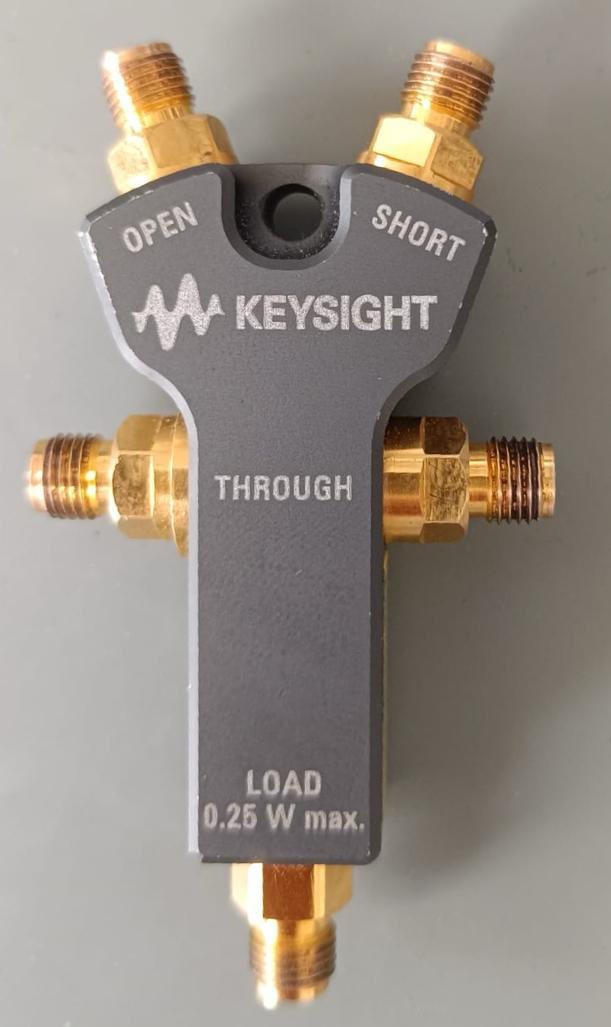
\includegraphics[width=0.25\textwidth]{Pictures/Keysightkallibrierung.jpg}
    \caption{Kalibrierungsgerät am Keysight FieldFox}
\end{figure}
\clearpage
 
Die Kalibrierung wird am Keysight FieldFox durchgeführt. Sie erfolgt über sieben Schritte, die vom Gerät angeleitet werden. Danach ist das Gerät bereit für die Messung.
\subsection{Verfizierung der Qualität der SOLT-Kalibrierung}
Unter Beibehaltung des Messaufbaus werden nun die S-Parameter, der bei der Kalibrierung verwendeten Kabel, betrachtet. Ist die Kalibrierung gelungen sollte unter optimalen Bedingungen bei den Streuparametern keine Dämpfung mehr angezeigt werden, da die Kalibrierung die Kabeldämpfung herausrechnet. In unserem Fall zeigt die Messung eine kleine Abweichung, ist jedoch sehr nahe am Optimum. Es ist daher keine erneute Kalibrierung von Nöten.

\subsection{Messen der S-Paramter}
Nach der Kaliebrierung werden die S-Paramater der Schaltung gemessen. Der für den direkten Vergleich relevante S-Parameter ist S21. Dieser
ist in Abbildung 4.4 dargestellt.
\begin{figure}[h]
    \centering
    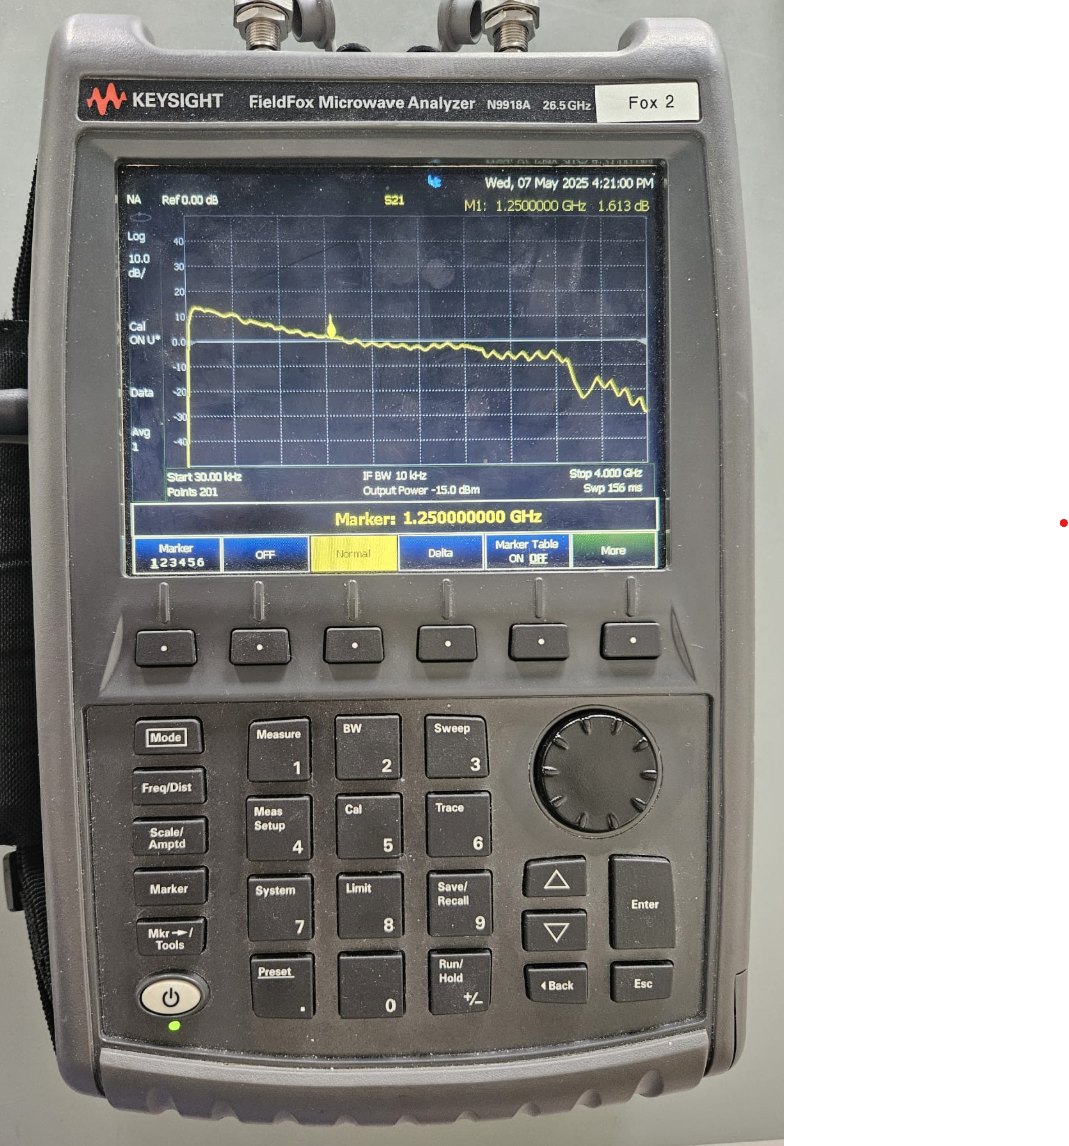
\includegraphics[width=0.5\textwidth]{Pictures/SParameterrichtig.png}
    \caption{S-Paramter S21}
\end{figure}
\clearpage




\section{Vergleich zur Simulation}
Im Versuch konnten wir ein Gain von 1.613 dB erreichen. Erwartet wurde der simulierte Gain von etwa 11.3 dB.
Die Abweichung kann auf verschiedene Faktoren zurückgeführt werden:
\begin{itemize}
    \item Die verwendeten Bauteile weichen von den idealen Werten ab und sind teilweise nicht für Hochfrequenztechnik geeignet.
    \item Die Induktivitäten und Kapazitäten der Leiterbahnen werden nicht in der Simulation berücksichtigt.
    \item Temperturschwankungen verschieben den Arbeitspunkt des Transistors
    \item Messungenauigkeite des Spektrumanalysators 
\end{itemize}

\clearpage
